\section{Experiments}
\vspace{-1ex}
\label{section:experiments}
\sam{Mettre expérience interprétation et sensibilité au bruit en appendice, améliorer l'interprétation des résultats}
For conciseness, several experiments are relegated in appendix: 

\begin{enumerate}
    \item \textbf{TS-LDDMM representation identifiability, \Cref{appendix: identifiability}:} On synthetic data, we evaluate the ability of our method to retrieve the parameter $v_0^*$ that encodes the deformation $\varphi^{\{v_0^*\}}$ acting on a time series graph $\msg$ by solving the geodesic shooting problem \eqref{eq:relaxation} between $\msg$ and $\varphi^{\{v_0^*\}}.\msg$.
     \textbf{Results} show that TS-LDDMM representations are identifiable or weakly identifiable depending on the velocity field kernel $K_G$ specification.
  
    \item \textbf{Robustness to irregular sampling, \Cref{appendix: robustness}:} We compare the robustness of TS-LDDMM representation with 9 URL methods handling irregularly sampled multivariate time series on 15 shape-based datasets (7 univariates \& 8 multivariates).
     We assess methods' classification performances under regular sampling (0\% missing rate) and three irregular sampling regimes (30\%, 50\%, and 70\% missing rates), according to the protocol depicted in \cite{kidger2020neural}.
      \textbf{Results} show that our method, TS-LDDMM, outperforms all methods for sampling regimes with missing rates: 0\%, 30\%, and 50\%.
      %{\color{red} J'enlèverai cette phrase ou je développerai en Appendix : The performance decrease of the Kernel-SVC based on TS-LDDMM representation is sensibly due to the misspecification of its regularization parameter.}
    
    \item \textbf{Classification benchmark on regularly sampled datasets, \Cref{appendix: shape_classification}:} We compare performances of a kernel support vector machine (SVC) algorithm based on TS-LDDMM representation with 3 state-of-the-art classification methods from shape analysis on 15 shape-based datasets (7 univariates \& 8 multivariates). \textbf{Results} show that the TS-LDDMM-based method outperforms other methods (best performances over 13 datasets), making TS-LDDMM representation relevant for time series shape analysis.
    
    \item \textbf{Noise sensitivity for learning the reference graph, \Cref{appendix: noise sensitivity}:} We evaluate the noise sensitivity of TS-LDDMM and Shape-FPCA \cite{wu2024shape} for learning the reference graph on a synthetic dataset and for several levels of additive Gaussian noise. \textbf{Results} show that both methods are sensitive to noise. However, TS-LDDMM preserves the overall shape while shape-FPCA alters the shape depending on the noise level. 
\end{enumerate}

\begin{figure}
  \centering
  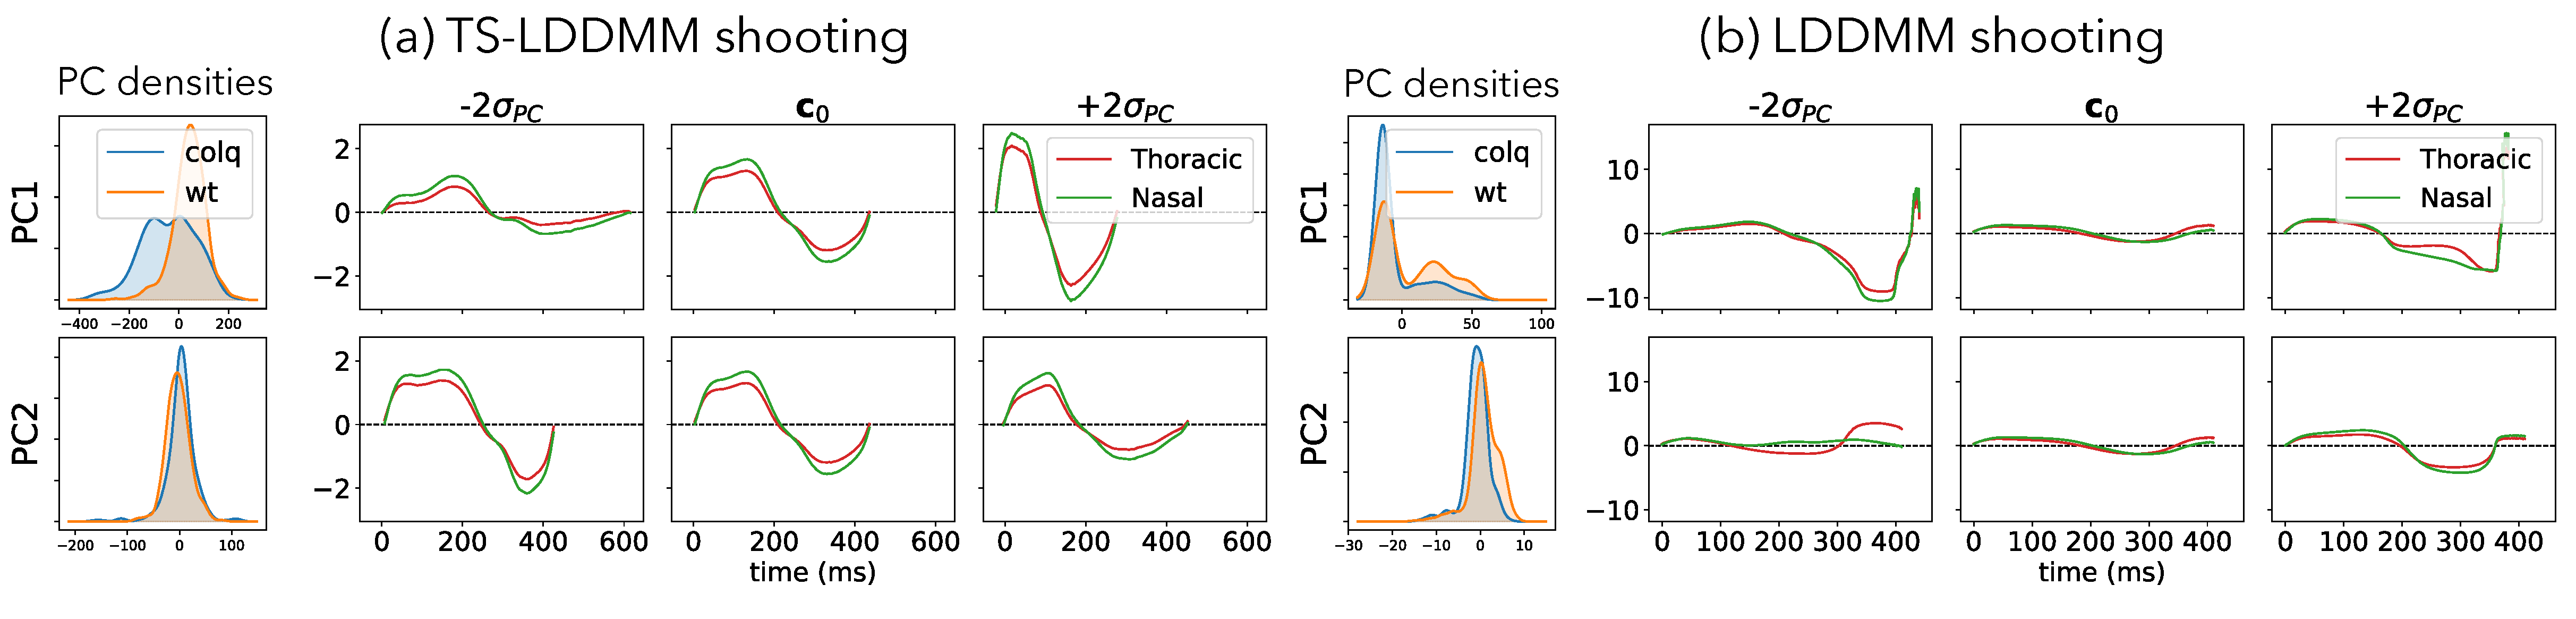
\includegraphics[width=\linewidth]{pictures/shooting before/shooting before.pdf}
  \caption{Analysis of the two principal components (PC) related to mice ventilation before exposure with TS-LDDMM representations \textbf{(a)}, and LDDMM \textbf{(b)}. In both cases and for all PC, the left plot displays PC densities according to mice genotype and right plot displays deformations of the reference graph $\mathbf{c}_0$ along each PC.}
  \label{fig:exp1}
  \vspace{-1.5em}
\end{figure}

\begin{figure*}[t]
  \centering
  \begin{subfigure}[b]{0.15\textwidth}
    \centering
    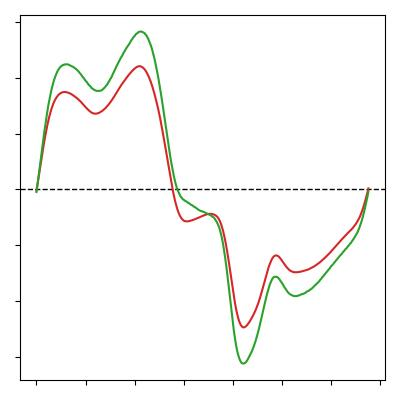
\includegraphics[width = \textwidth]{pictures/exp_1_cycle_example.jpeg}
    \caption{ColQ cycle}
    \label{fig:colq-cycle}
  \end{subfigure}
  \begin{subfigure}[b]{0.15\textwidth}
    \centering
    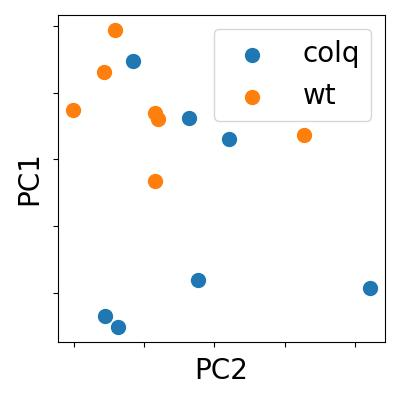
\includegraphics[width = \textwidth]{pictures/exp_1_scatter.jpeg}
    \caption{PC1 vs PC2}
    \label{fig: pcs-scatter}
  \end{subfigure}
  \begin{subfigure}[b]{0.15\textwidth}
    \centering
    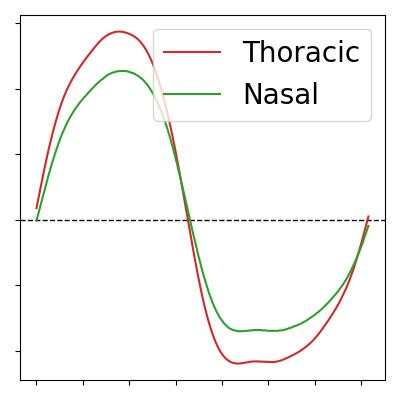
\includegraphics[width = \textwidth]{pictures/exp_1_wt.jpeg}
    \caption{WT cycle}
    \label{fig:wt-reference}
  \end{subfigure}
  \caption{\textbf{(a)} a ColQ respiratory cycle sample. \textbf{(b)} Referent respiratory cycle of individual mouse $\mathbf{c}_0^j$ in the TS-LDDMM PC1-PC2 coordinates system of $\mathbf{c}_0$. \textbf{(c)} a WT respiratory cycle sample.}
  \vspace{-1.5em}
\end{figure*}
\vspace{-1ex}
\subsection{Interpretability: mice ventilation analysis}
\label{section:interpretability}
\vspace{-1ex}
This experiment highlights the \textit{interpretability} of TS-LDDMM representation for studying the inter-individual variability in biomedical applications. We consider a time series dataset monitoring the evolution of mice's nasal and thoracic airflow when exposed to a drug altering respiration \cite{nervo2019respiratory}.
The dataset includes recordings of 7 control mice (WT) and 7 mutant mice (ColQ) with an enzyme deficiency. The enzyme is involved in the respiration regulation, and the drug inhibits its activity. For each mouse, airflows were monitored for 15 to 20 minutes before the drug exposure and then for 35 to 40 minutes. A complete description of the dataset is given in the \Cref{appendix:mouse_dataset}.
\vspace{-1ex}

\paragraph{Experimental protocol.} 
We considered two experimental scenarios; the first focuses on mice ventilation before exposure to explore the inter-individual and genotype-specific variabilities. The second focuses on whole recordings to analyze the evolution of mice's ventilation after drug exposure. In both cases, the baseline protocol consists of first extracting $N$ respiratory cycles from the datasets with the procedure described in \cite{germain2023unsupervised}. Then, learning the referent respiratory cycle $\mathbf{c}_0$ and the representations  of respiratory cycles $(\bm{\alpha}_0^j)_{j \in [N]}$ by solving \eqref{eq:general_optimization_problem} using TS-LDDMM. $\bm{\alpha}_0^j$ being the momentum of the initial velocity field of the geodesic encodings the diffeomorphisms mapping $\mathbf{c}_0$ to the $j^{th}$ respiratory cycle. Finally, performing a Kernel-PCA on the initial velocity fields~\eqref{eq:def_v0} belonging to $\msv$ and encoded by the pairs $(\bm{\alpha}_0^j,\mathbf{c}_0)_{j \in [N]}$. The first experiment includes $N_1 = 700$ cycles collected before exposure. The second experiment includes $N_2 = 1400$ cycles with 25\% (resp. 75\%) before (resp. after) exposure. We also performed the first experimental scenario with LDDMM representation, and \Cref{appendix: mice_exp_setting} describes the settings of both methods. Essentially, varifold losses are identical for both methods, and the velocity field kernels are set to encompass time and space scales. in addition, In addition, \Cref{appendix: mice_exp_setting}  presents a comparison between TS-LDDMM and Shape-FPCA on the second scenario. 
\vspace{-1ex}

\paragraph{Geodesic shooting along principal component directions.}
Any principal component (PC), noted $v_0^{pc}$, from a kernel-PCA in $\msv$, is itself an initial velocity field encoded by a pair $(\mathbf{c}_0, \bm{\alpha}_0^{pc})$. PCs encode the principal axis of deformations, and it is possible to shoot along the geodesic they encode with the differential equations \eqref{eq:integration}, enabling interpretation of the main sources of deformations.
\vspace{-1ex}

\paragraph{Mice ventilation before exposure.}
We focus on the analysis of the two first Principal Components (PC) for TS-LDDMM (\Cref{fig:exp1}a) and LDDMM (\Cref{fig:exp1}b). Looking at the geodesic shooting along PCs, \Cref{fig:exp1} shows that principal components learned with TS-LDMM lead to deformations that remain respiratory cycles. In contrast, deformations learned with LDDMM are challenging to interpret as respiratory cycles. The LDDMM velocity field kernel is a Gaussian anisotropic kernel that accounts for time and space scales; however, the entanglement of time and space dimensions in the kernel does not guarantee the graph structure, and it makes the convergence of the method complex (relative varifold loss error: TS-LDDMM: 0.06, LDDMM: 0.11).

Regarding TS-LDDMM \Cref{fig:exp1}a, its PCs refer to deformations directions carrying different physiological meanings. Indeed, the geodesic shooting along these directions indicates that PC1 accounts for variations of the total duration of a respiratory cycle, while PC2 expresses the trade-off between inspiration and expiration duration. In addition, the distribution of ColQ respiratory cycles along PC1 is wider than in WT mice, indicating that the adaptation of mutant mice to their enzyme deficiency is variable. This observation can also be seen in \Cref{fig: pcs-scatter} where a referent respiratory cycle $\mathbf{c}_0^j$ is learned by solving \eqref{eq:general_optimization_problem} for each mouse and is encoded in the (PC1,PC2) coordinate system of $\mathbf{c}_0$ by registration \eqref{eq:geodesics_shooting}. Indeed, the average respiratory cycles of ColQ mice are more spread out than WT mice's. Going back to the densities of PC1, ColQ mice distribution has a heavier tail toward negative values compared to WT mice. When shooting in the opposite direction of PC1, we can observe that the inspiration is divided into two steps. Congruently with \cite{germain2023unsupervised}, such inspirations indicate motor control difficulties due to enzyme deficiency. \Cref{fig:colq-cycle} is an example of ColQ respiratory cycle with negative PC1 coordinate.

\begin{figure*}[t]
  \centering
  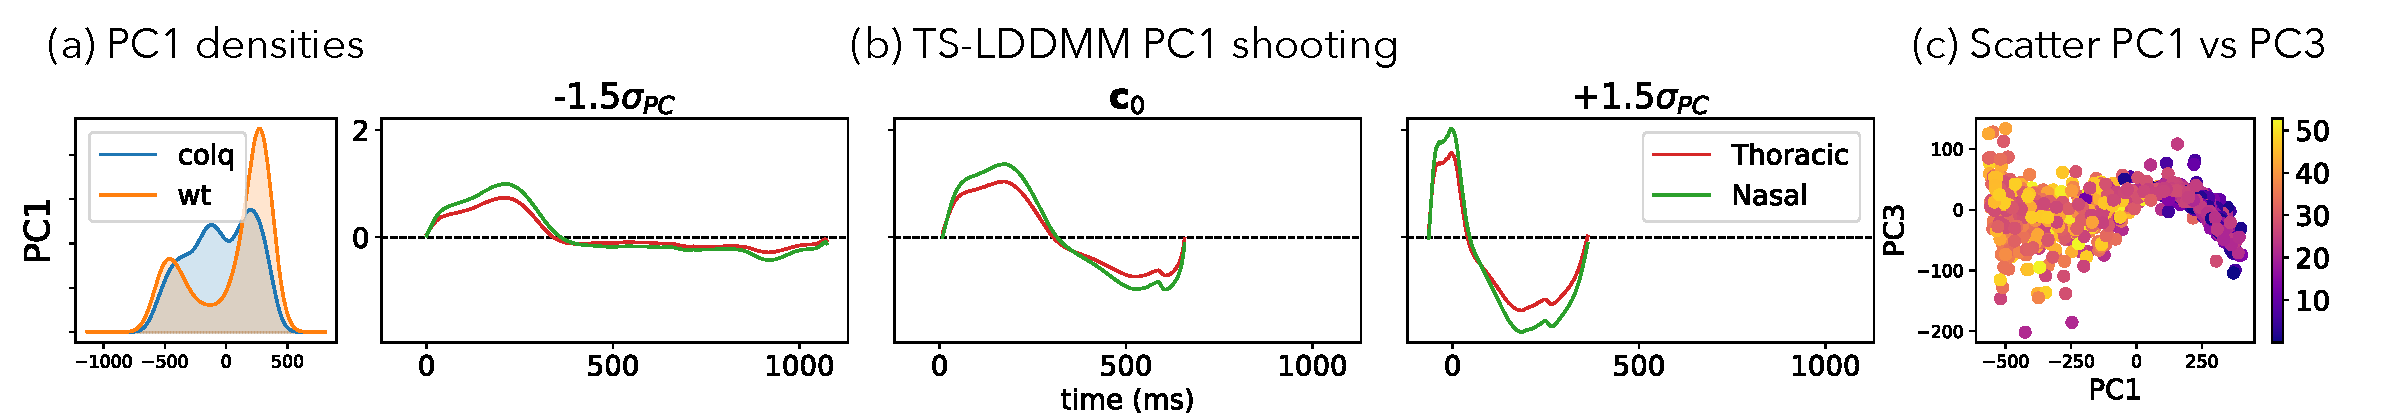
\includegraphics[width=\linewidth]{pictures/exp after/exp after.pdf}
  \caption{Analysis of the first Principal Component (PC1) related to mice ventilation before and after exposure with TS-LDDMM representations. \textbf{(a)} displays PC densities per mice genotype, \textbf{(b)} illustrates deformations of the reference respiratory cycle $\mathbf{c}_0$ along PC1, and \textbf{(c)} displays all respiratory cycles with respect to time in PC1 and PC3 coordinates}
  \label{fig:exp_2_PCA}
  \vspace{-1.5em}
\end{figure*}
\vspace{-1ex}

\paragraph{Mice ventilation evolution after drug exposure.} 
This experiment focuses on the first principal components learned from TS-LDDDM representations of respiratory cycles randomly sampled before and after drug exposure. \Cref{fig:exp_2_PCA}a illustrates the geodesic shootings along PC1. Again, PC1 accounts for variations in respiratory cycle duration, but more importantly, it can be observed on the deformation at -1.5 $\sigma_{\text{PC}}$ the apparition of a long pause after inspiration. Congruently, \Cref{fig:exp_2_PCA}c indicates that pauses appear after drug exposure as cycles with negative PC1 values mainly occur after 20 minutes and present more variability along PC3. In addition, \Cref{fig:exp_2_PCA}b shows a bimodal distribution for WT mice with one of the peaks in the negative values. This peak was not observed in the previous experiment \Cref{fig:exp1}a. It indicates that pauses after inspiration are prevalent in WT mice after drug exposure. On the other hand, the distributions of ColQ mice's respiratory cycles along PC1 in both experiments are similar and account for the same deformation, suggesting that ColQ mice weakly react to the drug exposure as they already adapt their enzyme deficiency. 
\vspace{-1ex}

\paragraph{Experiment Conclusion.}
Analyzing mice ventilation with TS-LDDMM representation highlights the method's ability to create meaningful interaction between experts and the data. Indeed, combining statistical and visual results shows that main deformations carry physiological meaning, enabling the characterization of some mice genotypes and the effects of drug exposure. 

\iffalse
\paragraph{Protocol.} For both experiments and representations (TS-LDDMM and LDDMM), we derive the reference respiratory cycle's graph $S_0$ and the representations $(\alpha_j)_{j\in[N]}$ related to $N$ respiratory cycles extracted according to the procedure \cite{germain2023unsupervised} by solving  \eqref{eq:general_optimization_problem}.
 Then, we perform a kernel PCA on the initial velocity field $\left(v_0(\alpha_j,S_0)\right)_{j\in[N]}\in \msv^{N_1}$ defined in \eqref{eq:def_v0} to breathing behavior.
  The first experiment includes $N_1 = 700$ respiratory cycles collected before exposure. The second experiment includes $N_2 = 1400$ respiratory cycles with 25\% (resp. 75\%) before (resp. after) exposure.
   \Cref{appendix: mice_exp_setting} describes methods settings.
    Essentially, varifold losses are identical for both methods, and the velocity field kernels are set to encompass time and space scales. 

    
    \vspace{-1ex}
\paragraph{Breathing behaviors before exposure.}
 We focus on the analysis of the two first Principal Components (PC) for TS-LDDMM (\Cref{fig:ts-lddmm shooting}), and LDDMM (\Cref{fig:lddmm shooting}).
  A respiratory cycle is an inspiration (positive flow) followed by an expiration (negative flow); \Cref{fig:wt-reference} displays an example of \textbf{wt} mouse respiratory cycle.
   \Cref{fig:exp1} shows that principal components learned with TS-LDMM lead to deformations that remain respiratory cycles, while deformations learned with LDDMM are challenging to interpret as respiratory cycles.
   The LDDMM velocity field kernel is a Gaussian anisotropic kernel that accounts for time and space scales; however, the entanglement of time and space dimensions in the kernel does not guarantee the graph structure, and it makes the convergence of the method difficult (relative varifold loss error: TS-LDDMM: 0.06, LDDMM: 0.11).
    Regarding TS-LDDMM, \Cref{fig:ts-lddmm shooting} shows its principal components refer to different types of deformations.
     By interpreting \Cref{fig:ts-lddmm shooting}: PC1 accounts for time warping, PC2 expresses the trade-off between inspiration and expiration duration.
      Compared to \textbf{wt} mice, the distribution of \textbf{colq} mice feature along the PC1 axis has a heavy left tail, and the associated deformation (-2 $\sigma_{\text{PC}}$) shows an inspiration with two peaks.
       \Cref{fig:colq-cycle} shows an example of such respiratory cycles, which may be caused by motor impairment due to enzyme deficiency \cite{germain2023unsupervised}.
        Finally, \Cref{fig: pcs-scatter} shows that PC1 and PC2 capture the main differences between the two groups as their respective reference graphs $S^j$ are located in different parts of the space. 

\begin{figure*}[t]
  \centering
  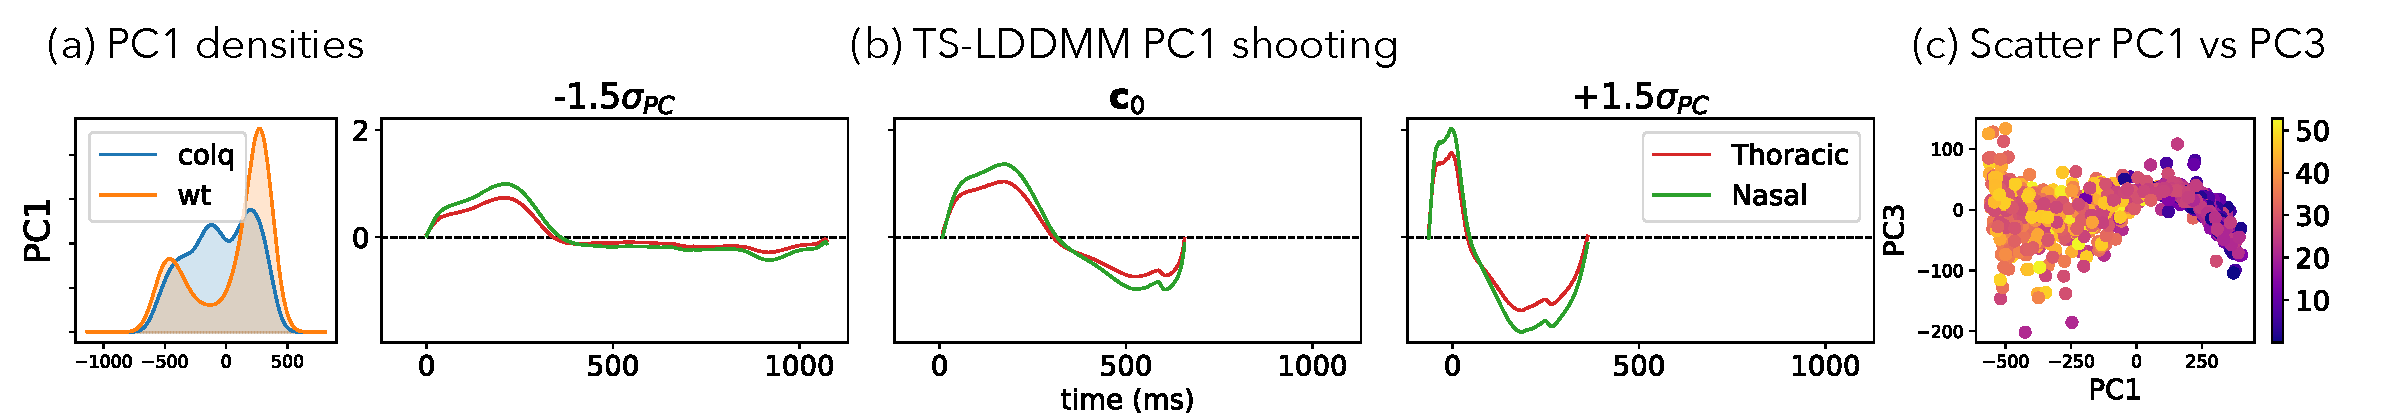
\includegraphics[width=0.95\linewidth]{pictures/exp after/exp after.pdf}
  \caption{Analysis of the first Principal Component (PC1) related to mice ventilation before and after exposure with TS-LDDMM representations. \textbf{(a)} displays PC densities per mice genotype, \textbf{(b)} illustrates deformations of the reference respiratory cycle $\mmathbf{c}_0$ along PC1, and \textbf{(c)} displays all respiratory cycles with respect to time in PC1 and PC3 coordinates}
  \label{fig:exp_2_PCAold}
  \vspace{-1.5em}
\end{figure*}
\vspace{-1ex}
\paragraph{Breathing behaviors' evolution after exposure to the irritant molecule} 
TS-LDDMM representation features are learned on a dataset that includes respiratory cycles before and after exposure.
 \Cref{fig:exp_2_PCA} displays the first principal component PC since it encodes the effect of the irritant molecule as depicted in \Cref{fig:exp_2_PCA}-C) (the exposure occurs at 20 minutes). \Cref{fig:exp_2_PCA}-B) shows that the deformation (-1.5 $\sigma_{\text{PC}}$) leads to longer respiratory cycles that include a pause between inspiration and expiration as observed in \cite{germain2023unsupervised}.
  Conjointly, \Cref{fig:exp_2_PCA}-A) shows a bimodal distribution for \textbf{wt} mice whereas \textbf{wt}' distributions before exposure were unimodal (\Cref{fig:ts-lddmm shooting}). Indeed, the irritant molecule inhibits the action of the deficient enzyme, \textbf{wt} mice strongly react to the irritant molecule, whereas \textbf{colq} mice better adapt due to their deficiency \cite{germain2023unsupervised}.
%   \vspace{-1ex}
% \paragraph{Result summary.} By comparing the shape of individual respiratory cycles, we show that TS-LDDMM features can encode genotype distinctive breathing behaviors and their evolution after exposure to the irritant molecule contrary to LDDMM \cite{glaunes2008large}. 
% \vspace{-1ex}
%Secondly, we compare breathing behaviors before and after exposure to observe the impact of the irritant molecule.
% We follow the same procedure as for before exposure, but we take $N_2=1400$ respiratory cycles extracted according 
% to the procedure CITE....
% In \Cref{fig:exp_2_PCA}, we focus on the first Principal Component (PC) since it encodes the effect of the irritant molecule as demonstrated on Figure \ref{fig:exp_2_PCA}-C) (exposure at time 20).
% We observe on \Cref{fig:exp_2_PCA}-B) that after exposure the mouse have longuer breath such that the expiration is longuer than inspiration.
%  Moreover, we deduce from Figure \ref{fig:exp_2_PCA}-A) that \textbf{colq} are more constant in their breath compared to \textbf{wt} after exposure.
%
% In Figure REF, we 
% also display the reference respiratory cycle S0 and its deformations in the principal component directions.
%  Additionally, we learn each mouse's reference respiratory cycle and represent them in the first and third PC coordinates system in Figure REF. 

\fi